%% vi: set tabstop=2, set textwidth=80
\documentclass[a4paper,11pt]{article}

\usepackage{homework}
\usepackage{graphicx, subfigure}
\usepackage{verbatim}
\usepackage{algorithm, algorithmic}
\usepackage{amsmath, amsthm, amssymb}
\usepackage[english]{babel}

\title{Locate My Plate \\ A License Plate Localisation System}

\date{June 24, 2009}

\begin{document}

\maketitle
\section{Introduction}
This report describes the implementation of a robust, real-time License Plate
Localisation system (LPL) \cite{dlagnekov_thesis, zhang}. We analyze which
characteristic features are important for license plate localisation. Using
supervised learning, the system generates a cascading classifier which consists
of layers that each hold one strong classifier. A strong classifier is a linear
function of several weak classifiers obtained by boosting. Each weak classifier
is a feature which describes characteristics of a license plate. Section
\ref{sec:data} describes the data used for our experiments. Section
\ref{sec:feat} describes the features and how they are generated. Next the
training and classification of weak-, strong- and cascading classifiers are
both explained. Finally the results are shown and we come to the conclusions.

\section{Dataset} \label{sec:data}
The dataset used is obtained from \cite{dlagnekov_dataset}. It contains $246$
car images with a resolution of approximately $640\times480$. The images are
annotated on location and size of the license plate and were rescaled by
$50\%$. The dataset is divided in a train-, test- and validation set with
$159$, $40$ and $47$ images respectively.


\section{Features} \label{sec:feat}
The core of the LPL system consists of features as described by
\cite{dlagnekov_thesis, zhang,naturaltext}. Features are image filters applied
on a certain type of image (e.g. an $x$-derivative) see Figure \ref{fig:feature}.
Formally a feature $f$ is a tuple $\langle i, B, o \rangle$ defined as:
\begin{itemize}
	\item{$i$, an index corresponding to the image type.}
	\item{$B$, the set of blocks where each block $b \in B$ contains a sign
	$b_s \in \{-1,1\}$ indicating subtraction or addition of that block and
	positions $b_{pa},b_{pb} \in [0,1]$, determine the relative block position
	within the feature.}
	\item{$o$, the orientation of the feature blocks: horizontal or vertical.}
\end{itemize}
\begin{figure}[!ht]
\centering
\subfigure[The original image.]{
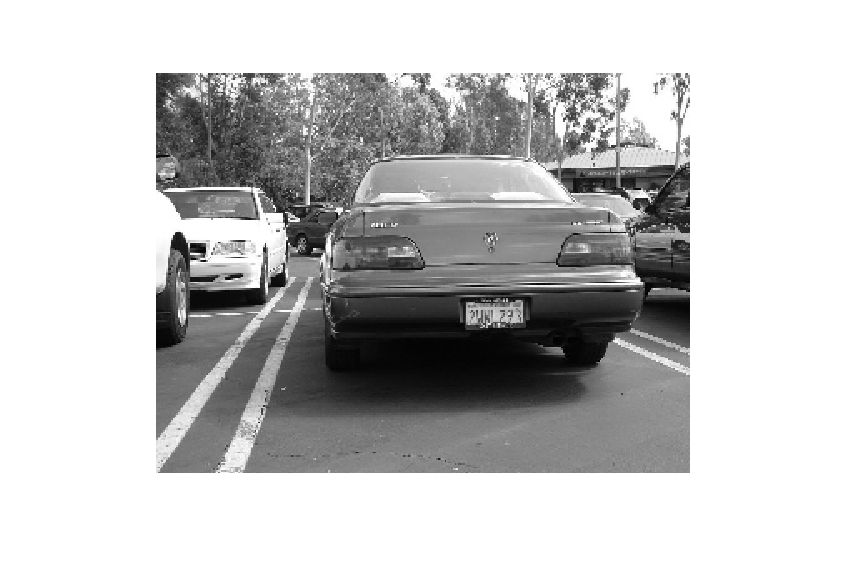
\includegraphics[height=3.5cm]{img/original}
\label{fig:a}
}
\subfigure[The feature.]{
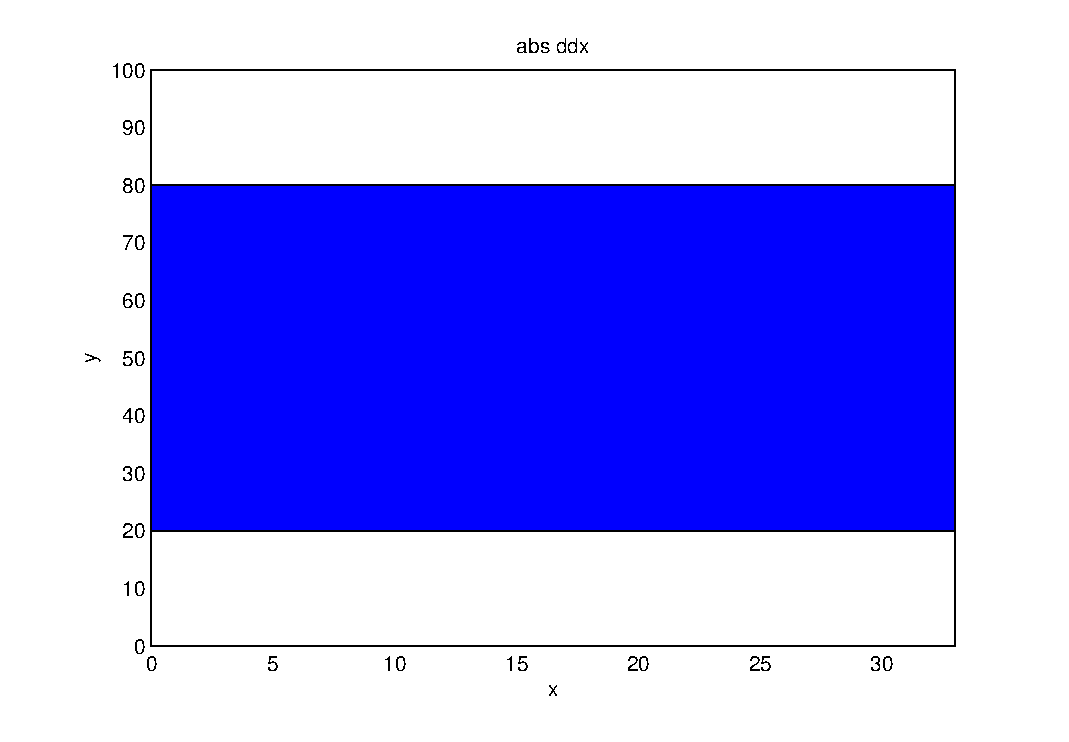
\includegraphics[height=3.5cm]{img/feature}
\label{fig:b}
}
\subfigure[The feature applied.]{
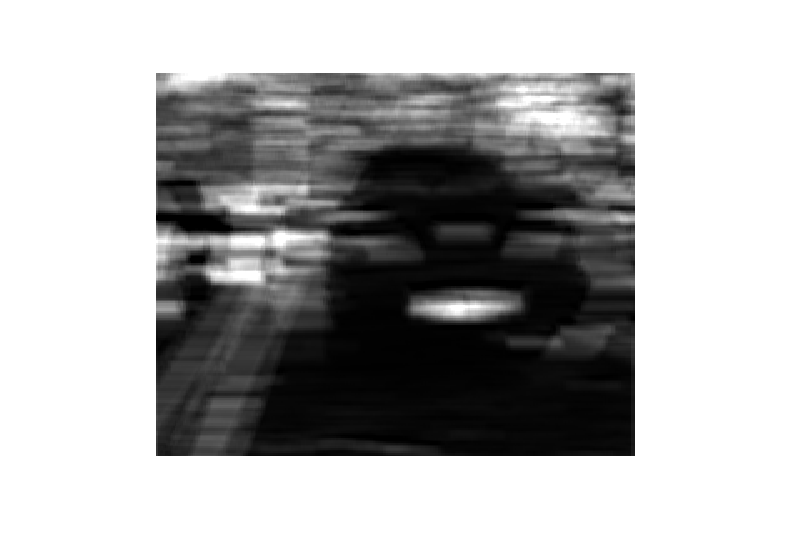
\includegraphics[height=3.5cm]{img/featureapplied}
\label{fig:c}
}
\caption{A horizontal, second order $x$-derivative feature with binary code
$01110$, consisting of three blocks applied to an image.}
\label{fig:feature}
\end{figure}
The feature value $f:x\mapsto\mathbb{R}$ of an image $x$ is shown in Algorithm
\ref{alg:value}.
\begin{algorithm}[!htb]
	\caption{featureValue($f$, $x$, $w$, $h$): Returns the image $V = f(x)$}
	\begin{algorithmic}[1]
	\REQUIRE The feature $f = \langle i, B, o \rangle$, the image $x$, the width $w$ and height $h$ of the feature.
	\medskip
	\STATE Initialize $V$ as an image with dimensions $D(x)-[w, h]$ consisting of zeros.
	\STATE Let $I$ be the $i^{th}$ image type of $x$.
	\IF {$o$ is horizontal}
		\STATE $I \leftarrow I^\top$
		\STATE Swap $w$ and $h$
	\ENDIF
	\STATE Let $B'$ be the set of blocks with rescaled coordinates using $w,h$.
	\FORALL {$b \in B'$}
		\STATE Let $X$ be the result of applying $b$ to $I$ while respecting $b_{pa}, b_{pb}$ alignment.
		\STATE $V \leftarrow V + b_s \cdot X$
	\ENDFOR
	\RETURN $V$
	\end{algorithmic}
\label{alg:value}
\end{algorithm}

\newpage
\subsection{Image Types} \label{sec:image}
For this report, the following image types were used.
\begin{itemize}
	\item{1st order derivative in both $x$ and $y$ directions.}
	\item{2nd order derivative in both $x$ and $y$ directions.}
\end{itemize}
Before applying the feature, the above image types are passed through an
absolute filter. By calculating an integral image per image type, the
featureblocks can be calculated very efficiently as each block calculation
requires four array access instructions \cite{viola}.

\subsection{Generation} \label{sec:gen}
By representing a feature as a binary string, the set $S$ of possible features
can be easily calculated:
$$S = \{b(x,n) | \forall x \in \{1,\ldots,(2^n-2)/2\}\},$$
where $b(x,n)$ represents $x$ as a binary string of length $n$ as the number of
segments. Note that binary strings $0_1,\ldots,0_n$, $1_1,\ldots,1_n$ and the
inverse binary strings are ignored. Each element in the binary string $s \in S$
represents the position and the sign of a feature segment. Adjacent segments
that share the same sign are merged together and are called a feature block.
This set of features is duplicated for each image type.

% \subsection{Optimization} \label{sec:opt}
% Features often share the same feature block dimensions. A feature can have
% multiple feature blocks of the same dimensions, because the feature is applied
% as an image filter.  To optimize this, the feature blocks are individually
% calculated for every position $(x,y)$, in the image $i$ and stored on its
% dimensions $(w_i,h_i)$ in a hash table $R_i$.


\section{Training} \label{sec:train}
The overall cascading classifier consists of three types of training. The first
type is the training of the weak classifiers using features. The second type is
a linear combination of one or more weak classifiers into a strong classifier
using a boosting algorithm. The third type is a cascading classifier
with a strong classifier on each layer.

\subsection{Weak Classifier} \label{sec:weak}
A weak classifier consists of a feature $f$, a threshold $t \in \mathbb{R}$ and
an operator $\circ \in \{<, >\}$ which separates positive and negative samples
according to the trainings set. After training, the weak classifier $C$
constructs a binary image $B = t \circ f(x)$, where $x$ is the image and $f$
the function that returns the value of the feature as described in Section
\ref{sec:feat}. The locations of the ones in $B$ correspond to the location of
possible license plates.

\subsection{Strong Classifier} \label{sec:strong}
By combining weak classifiers, a strong classifier can be formed. This is the
principle of boosting.  A strong classifier is constructed according to the
boosting algorithm adaboost, described by \cite{viola}. Adaboost is adaptive
with respect to the weak classifiers it selects. By keeping two sets of
weights, those on the weak classifiers ($\alpha$) and those on the training
samples. Classification is performed as follows:
\begin{displaymath}
C(x) = 
	\left\{ \begin{array}{ll}
		1 & \sum^N_{i=1} \alpha_i \big(t_i \circ_i f_i(x)\big) \ge \tau \sum^N_{i=1}\alpha_i \\
		0 & \textrm{otherwise}
	\end{array} \right.
\end{displaymath}
where $N$ is the number of weak classifiers as selected by the boosting
algorithm and $\tau \in [0,1]$ a threshold which allows for changing the false
positive- and detection rate.

\subsection{Cascading Classifier} \label{sec:casc}
The cascading classifier is the final classifier. This classifier is trained as
described in \cite{viola}. By specifying a false positive rate per layer, a
detection rate per layer and a false positive rate goal, the algorithm
constructs a cascade of strong classifiers using the training- and validation
set.  Algorithm \ref{alg:casc} shows the classification of an image using a
trained cascading classifier. The strong classifier $c_s \in C$ classifies
according to Section \ref{sec:strong}, while respecting the previous false
positives and true positives only. This results in a binary image $B'$ which is
logically `anded' with the previous binary image $B$ resulting in less false
positives after each iteration.
\begin{algorithm}[!htb]
	\caption{cascadingClassify($C$, $x$, $w$, $h$): Returns the binary image $B$ of $x$}
	\begin{algorithmic}[1]
	\REQUIRE $C$ the cascading classifier, $x$ the image, $w,h$ the dimensions of the features
	\medskip
	\STATE Initialize $B$ as an image with dimensions $D(x) - [w,h]$ consisting of ones.
	\FORALL {$c_s \in C$}
		\STATE $B' \leftarrow c_s(x|B)$
		\STATE $B \leftarrow B \land B'$
	\ENDFOR
	\RETURN $B$
	\end{algorithmic}
\label{alg:casc}
\end{algorithm}

\section{Results} \label{sec:res}
For our experiments we trained the cascading classifier using $fp = 0.99, d =
0.999, fp_{min} = 0.001$ for the false positive rate, detection rate and
minimal false positive rate respectively. Furthermore we generated features
consisting of $5$ segments. The total number of features generated was
$\frac{(2^5-2)}{2}\cdot 2 \cdot 4 = 120$. The final cascading classifier
contains five layers with $1, 4, 14, 7, 10$ features respectively. An example
of the cascading classifier is displayed in Figure \ref{fig:cascader}. To
illustrate how a layer is constructed, the strong classifier of layer 2 is
shown in Figure \ref{fig:strongclassify}. The confusion matrix on the test set
can be found in Table \ref{tab:conf}. 

\begin{figure}[!ht]
\centering
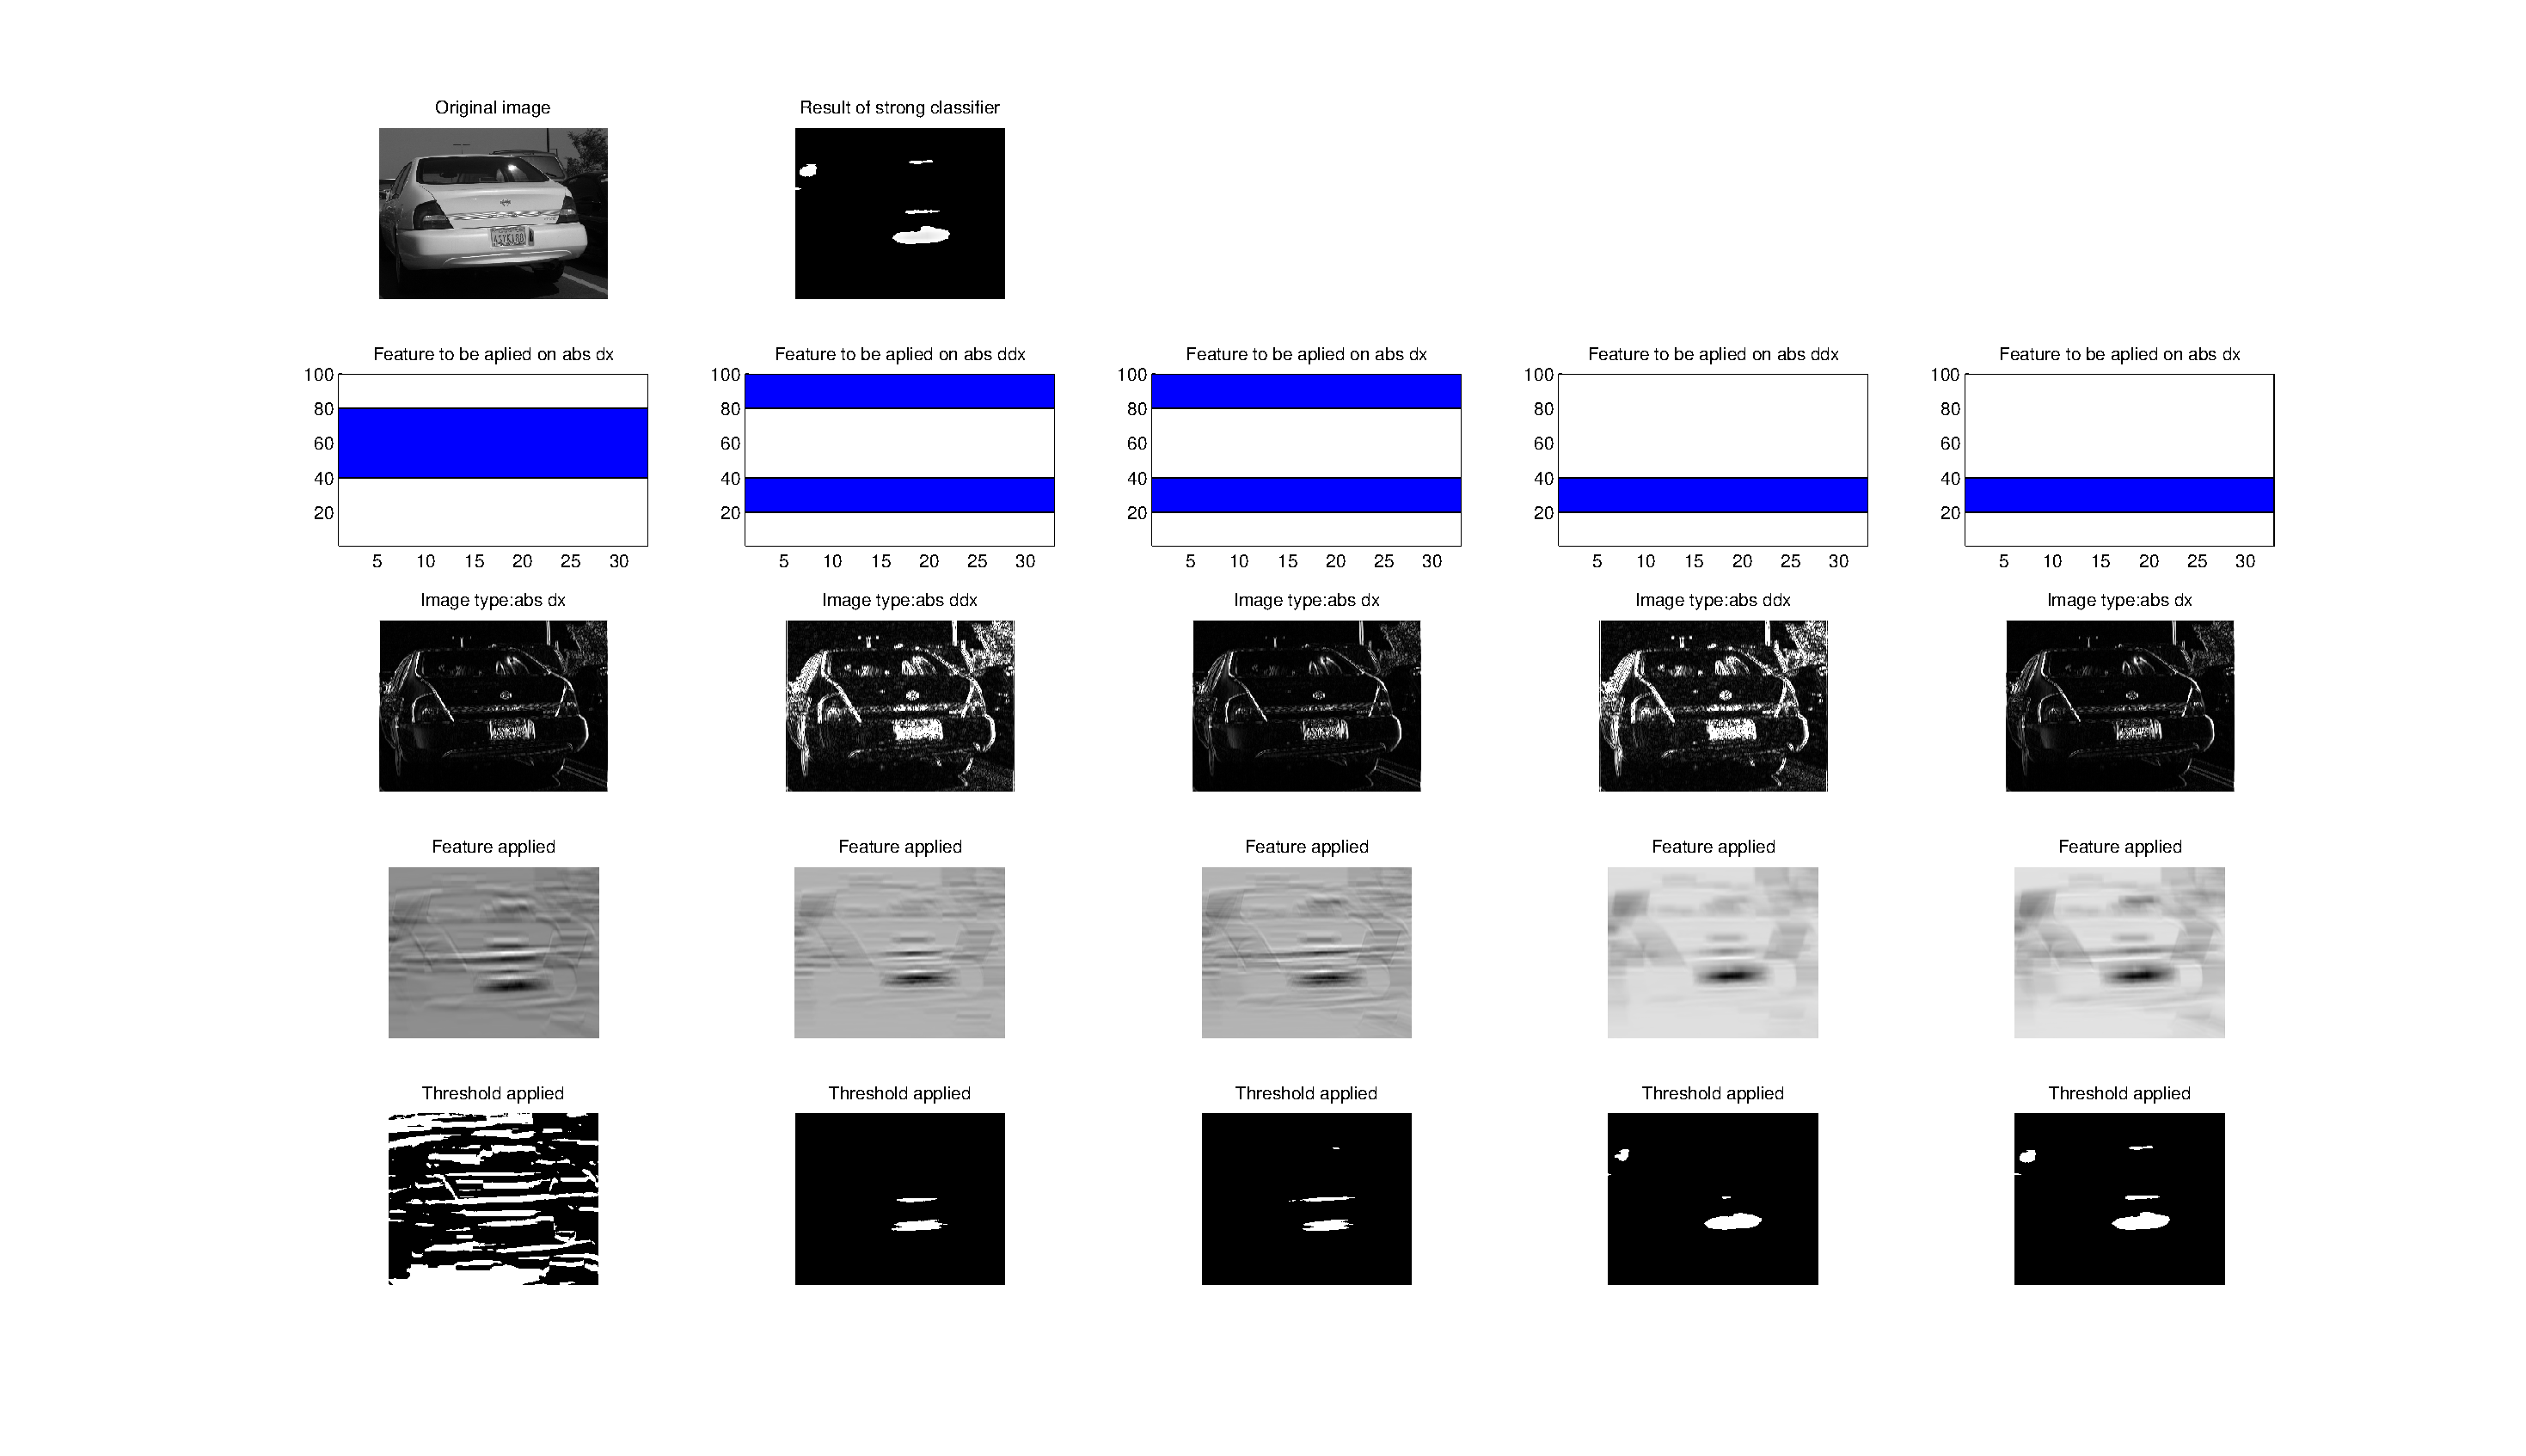
\includegraphics[width=16cm]{img/strongClassifier_layer2_img14}
\caption{Example of the strongclassifier in layer 2 with 4 features. The first
row shows the features, the second the image types, the third shows the
features applied to the image types and finally the bottom row shows the
thresholds.}
\label{fig:strongclassify}
\end{figure}

\begin{figure}[!ht]
\centering
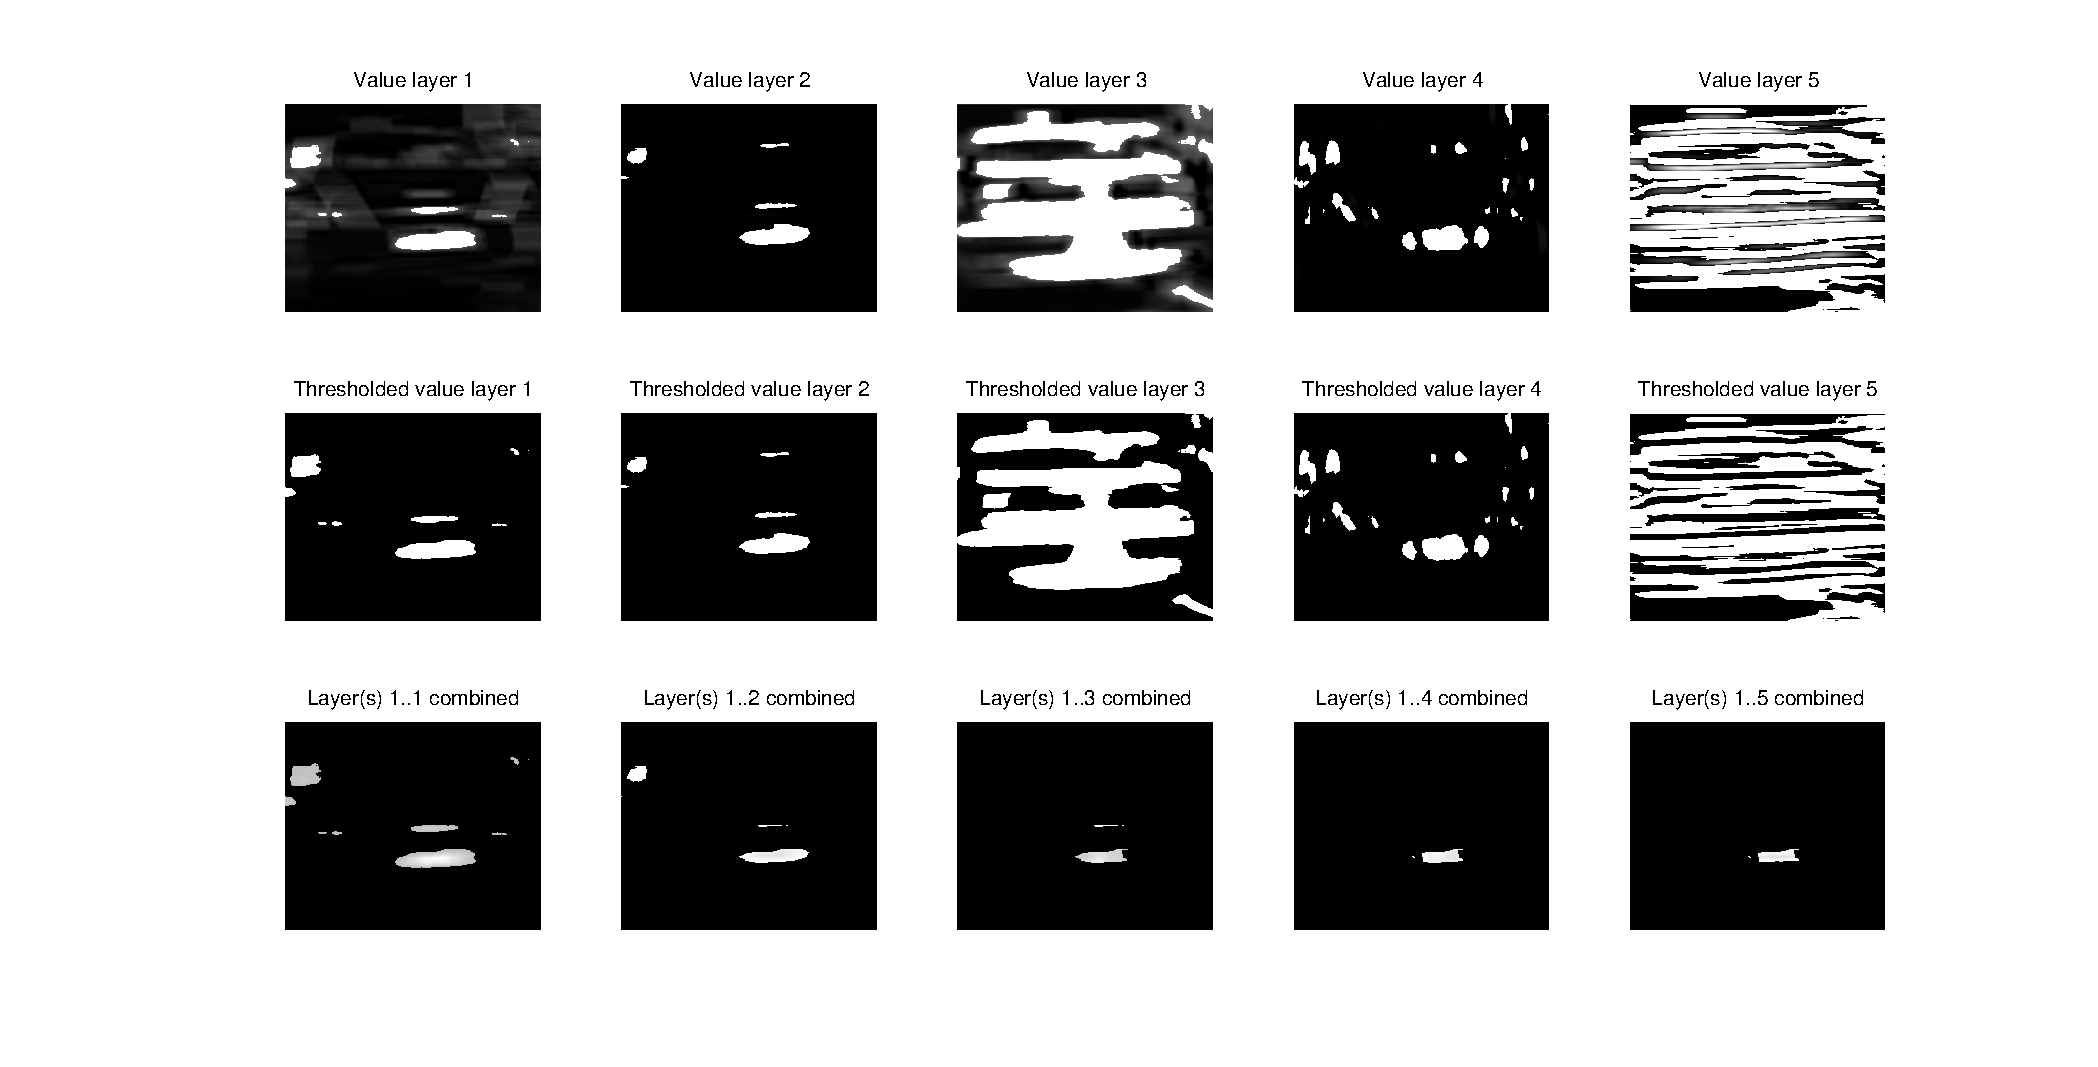
\includegraphics[width=16cm]{img/cascader_img14}
\caption{Example of the resulting cascading classifier with 5 layers. The first
row shows the values of the individual strong classifiers, the second row shows
the thresholded individual strong classifiers. The bottom row shows the actual
cascading result, each increasing layer more false positives are removed.}
\label{fig:cascader}
\end{figure}

\begin{table}[!ht]
\centering
\begin{tabular}{|l|l|}
\hline
$37$ & $166186$ \\
\hline
$3$  & $2399245$ \\
\hline
\end{tabular}
\caption{The confusion matrix of the test set.}
\label{tab:conf}
\end{table}
An overall detection rate of $0.925$ and false positive rate of $0.0648$ was
achieved. Figure \ref{fig:fprate} shows the averaged false positive rate per
layer in the cascading classifier. Note that we experimented with just four
image types as described in Section \ref{sec:image}, using more advanced image
types as described by \cite{naturaltext} would decrease the false positive rate
even further. A final result of the applied cascader can be found in Figure
\ref{fig:cascader}.
% TODO: (optional endresult, car with rectangle at license plate)
\begin{figure}[!ht]
\centering
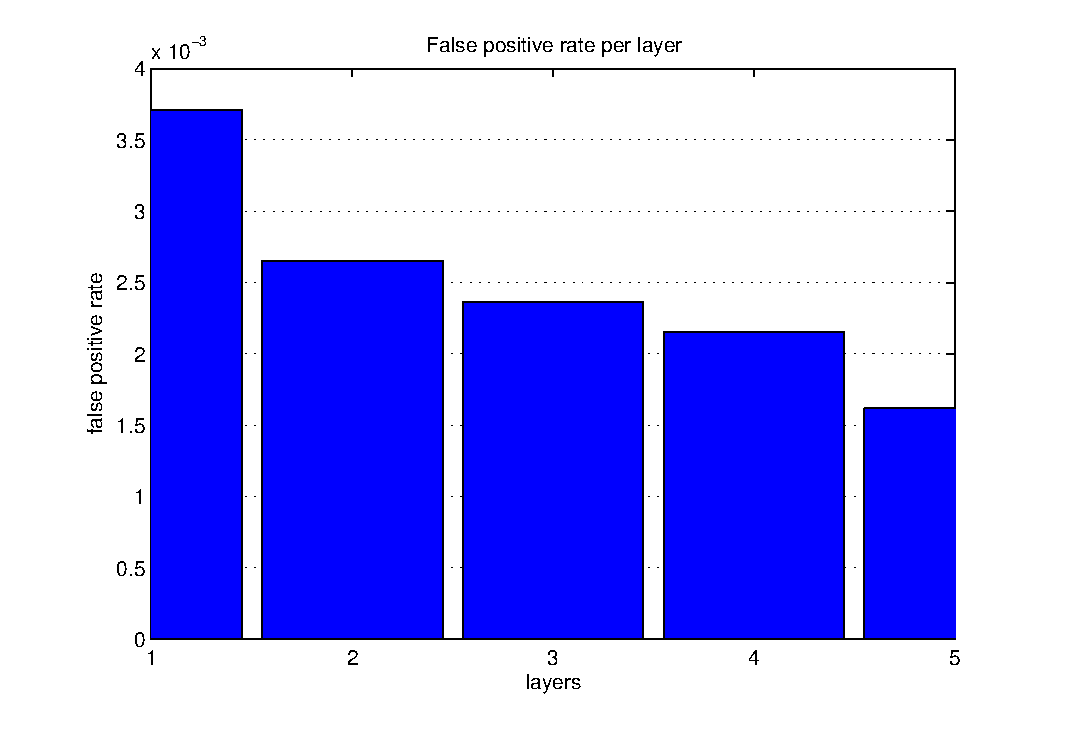
\includegraphics[height=7cm]{img/fprate}
\caption{The false positive rate per layer, averaged over the test set.}
\label{fig:fprate}
\end{figure}
\begin{figure}[!ht]
\centering
\subfigure[The original image]{
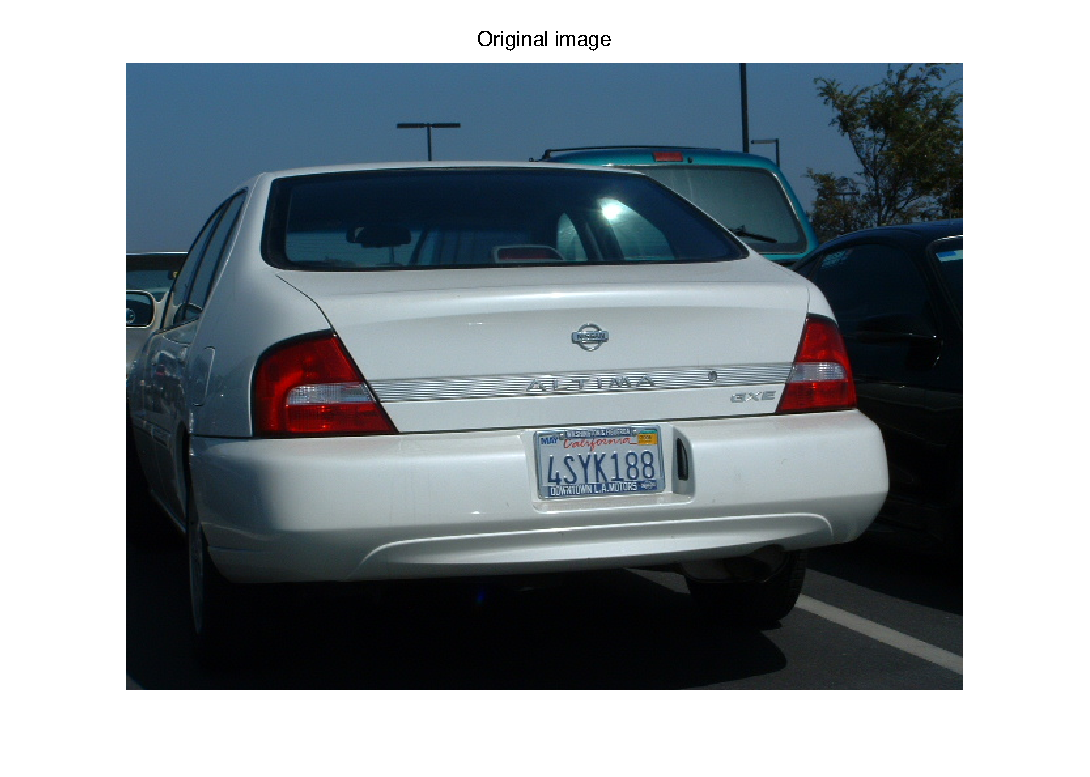
\includegraphics[height=5cm]{img/cascader_original}
\label{fig:x}
}
\subfigure[The cascader applied]{
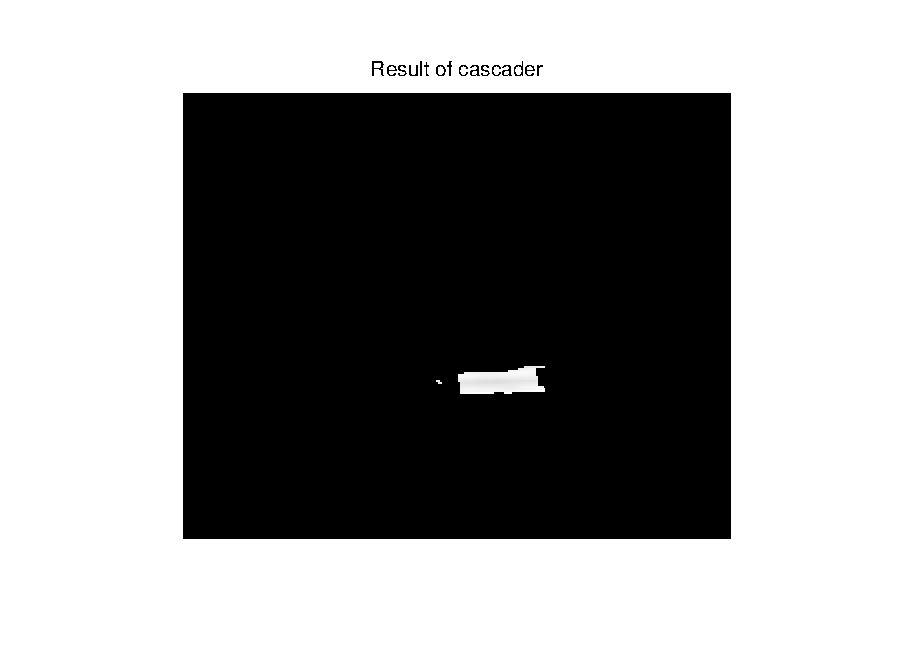
\includegraphics[height=5cm]{img/cascader_result}
\label{fig:y}
}
\caption{An original image of a car and the resulting binary image after cascading.}
\label{fig:result}
\end{figure}

\section{Conclusions} \label{sec:conc}
Given just four types of images, the cascading classifier performs very well.
With a detection rate of $0.925$ and false positive rate of $0.0625$ we can
conclude that License Plate Localisation can be effectively achieved using this
method. Even when no more sophisticated image types are used, the cascader
could be used by a License Plate Recognition system as the remaining false
positives can be filtered out by optical character recognition and the
characteristics of a license plate.
\newpage
\renewcommand\bibname{References}
\bibliography{references}
\bibliographystyle{IEEEtran}
\end{document}
